\documentclass[11pt]{article}
\usepackage[letterpaper]{geometry}
\usepackage{times}
\usepackage{verbatim}
\usepackage{graphicx}
\usepackage{float}
\usepackage{fullwidth}
\usepackage{amsmath}
\usepackage{amssymb}
\usepackage{fourier}
\usepackage{hyperref}
\graphicspath{{Images/}}
\title{ENGR-241 Passive Filters Lab}
\author{Jeremy Munson, Lauren Speirs \& Andrew Henrikson}
\geometry{top=.8in, bottom=.8in, left=.8in, right=.8in}

\setlength{\parindent}{0em}
\setlength{\parskip}{.5em}
\begin{document}
	\maketitle
	\subsection*{Overview}
	For this lab we designed and  constructed high and low pass filter circuits with RC components. We designed each circuit with a cutoff frequency of 10 KHz and used the signal generator to produce a 2V p-p sinusoidal waveform as the voltage source. We then swept the frequency between 1KHz and 100KHz and calculated the expected output voltage for given frequencies.
	\subsection*{Circuit Diagrams}
	Low Pass Filter: 
		\begin{figure}[H]
			\centering
			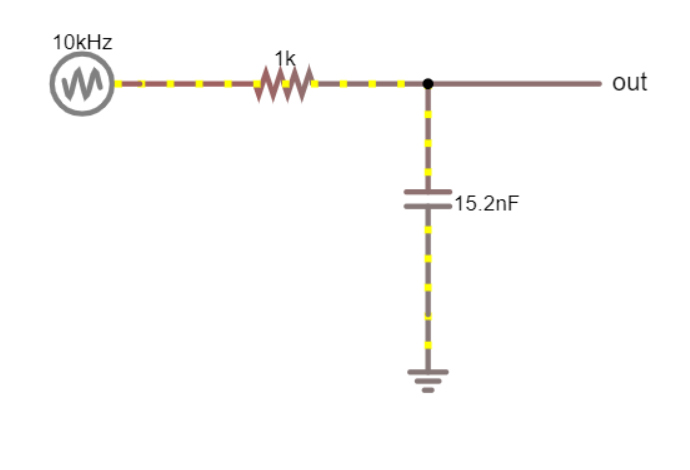
\includegraphics[width=3.5in]{images/low diagram.PNG}
		\end{figure}
		High Pass Filter:
		\begin{figure}[H]
		    \centering
		    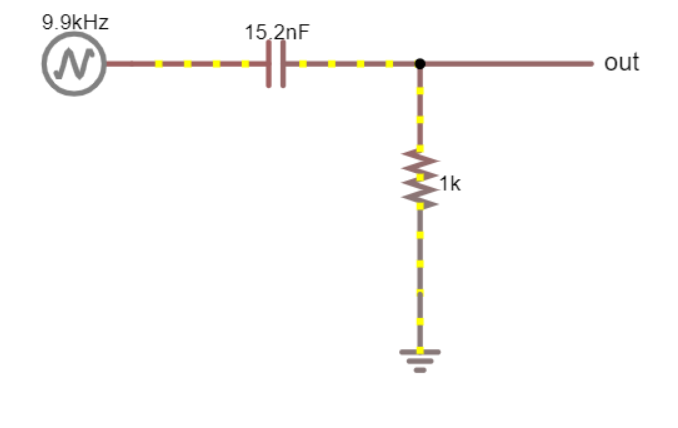
\includegraphics[width=3.5in]{images/high diagram.PNG}
		\end{figure}
	  
	\subsection*{Calculations}
	The calculations for this circuit were performed by finding the transfer function for three different frequencies between 1KHz and 100KHz and the calculated value along with the given input function to determine the expected output voltage of our high and low pass filters.
	\subsubsection*{1. Calculate the transfer of the given LPF circuit.}
	
	$H(j\omega)=\frac{\frac{1}{RC}}{j\omega+\frac{1}{RC}}$\\
	$\omega_{1}=1KHz\cdot 2\pi=2,000\pi rad/s$\\
	$\omega_{2}=10KHz\cdot 2\pi=20,000\pi rad/s$\\
	$\omega_{3}=100KHz\cdot 2\pi=200,000\pi rad/s$\\\\
	$H(j\omega_{1})=\frac{\frac{1}{1050\cdot 15.1 \cdot 10^{-9}}}{j\cdot 2000\pi+\frac{1}{1050\cdot 15.1 \cdot 10^{-9}}}$\\
	$H(j\omega_{1})=0.995075 \angle-5.6890^{\circ} $\\\\
	$H(j\omega_{2})=\frac{\frac{1}{1050\cdot 15.1 \cdot 10^{-9}}}{j\cdot 20,000\pi+\frac{1}{1050\cdot 15.1 \cdot 10^{-9}}}$\\
	$H(j\omega_{2})=0.708452 \angle-44.8909^{\circ} $\\	\\
	$H(j\omega_{3})=\frac{\frac{1}{1050\cdot 15.1 \cdot 10^{-9}}}{j\cdot 200,000\pi+\frac{1}{1050\cdot 15.1 \cdot 10^{-9}}}$\\
	$H(j\omega_{3})=0.09988 \angle-84.2678^{\circ} $\\
	
	\subsubsection*{2. Use these values to construct the time domain function for each frequency.}
	
	$V_{o(1)}=0.995075cos(2000\pi t-5.68903)V$\\
	$V_{o(2)}=0.70845cos(20,000\pi t-44.8909)V$\\
	$V_{o(3)}=0.09988cos(200,000\pi t-84.2678)V$\\
	
	\subsubsection*{3. Calculate the transfer of the given HPF circuit.}
	
	$H(j\omega)=\frac{j\omega}{j\omega+\frac{1}{RC}}$\\\\
	$\omega_{1}=1KHz\cdot 2\pi=2,000\pi rad/s$\\
	$\omega_{2}=10KHz\cdot 2\pi=20,000\pi rad/s$\\
	$\omega_{3}=100KHz\cdot 2\pi=200,000\pi rad/s$\\\\
	$H(j\omega_{1})=\frac{j\cdot 2000\pi}{j\cdot 2000\pi+\frac{1}{1050\cdot 15.1 \cdot 10^{-9}}}$\\
	$H(j\omega_{1})=0.099129 \angle84.311^{\circ} $\\\\
	$H(j\omega_{2})=\frac{j\cdot 20,000\pi}{j\cdot 20,000\pi+\frac{1}{1050\cdot 15.1 \cdot 10^{-9}}}$\\
	$H(j\omega_{2})=0.705759 \angle45.1091^{\circ} $\\\\	
	$H(j\omega_{3})=\frac{j\cdot 200,000\pi}{j\cdot 200,000\pi+\frac{1}{1050\cdot 15.1 \cdot 10^{-9}}}$\\
	$H(j\omega_{3})=0.995 \angle5.73224^{\circ} $\\\\
	
	\subsubsection*{4. Use these values to construct the time domain function for each frequency.}
	
	$V_{o(1)}=0.099129cos(2000\pi t+84.311)V$\\
	$V_{o(2)}=0.705759cos(20,000\pi t+45.1091)V$\\
	$V_{o(3)}=0.995cos(200,000\pi t+5.73224)V$\\
		\subsection*{Procedure}
	The circuits were simple to construct using the breadboard. Aside from constructing the circuit as normal, we used the LCR meter to select a capacitor to minimize to give us more accurate results between the ideal and observed circuits. After constructing the circuits, measurements were taken in the usual manner using the oscilloscope. We then swept the frequency through a large range with various waveforms to see the differentiating effect of the high pass filter. These outputs are shown below.
	
	
	Square Wave
	\begin{figure}[H]
		\centering
		\includegraphics[width=3.5in]{images/sq_wave HF.JPG}
		High Frequency
	\end{figure}
	
	\begin{figure}[H]
		\centering
		\includegraphics[width=3.5in]{images/sq_wave LF.JPG}
		Low Frequency
	\end{figure}
	\newpage
	Triangle Wave
	\begin{figure}[H]
		\centering
		\includegraphics[width=4in]{images/tri_wave HF.JPG}
		High Frequency
	\end{figure}
	
	\begin{figure}[H]
		\centering
		\includegraphics[width=4in]{images/tri_wave LF.JPG}
		Low Frequency
	\end{figure}
	
	\subsection*{Error Analysis}
	Our suggested values and measured values for our components used are shown in the table below. The percent error is also listed.
		\begin{table}[H]
		\def\arraystretch{1.2}%
		\centering
		\begin{tabular}{|l|l|l|l|}
			
			\hline
			Components       	& Suggested 		& Measured      	&\% Diff	\\ \hline
			Resistor  	    	& $1 k\Omega$		& $1.05 k\Omega$   & 5\%	     \\ \hline	
			Capacitor			& $16 n F$			& $15.15 nF$		& -5.3\%		\\ \hline
		\end{tabular}
	\end{table}
	\subsection*{Summary}
	
	\end{document}
